\documentclass{article}
\usepackage[utf8x]{inputenc}
\usepackage{ucs}
\usepackage{amsmath} 
\usepackage{mathtext}
\usepackage{amsfonts}
\usepackage{upgreek}
\usepackage[english,russian]{babel}
\usepackage{graphicx}
\usepackage{float}
\usepackage{textcomp}
\usepackage{hyperref}
\usepackage{geometry}
  \geometry{left=2cm}
  \geometry{right=1.5cm}
  \geometry{top=1cm}
  \geometry{bottom=2cm}
\usepackage{tikz}
\usepackage{ccaption}



\begin{document}
\pagenumbering{gobble}

\section*{Задачи:}
\subsection*{Часть A -- на оценку хор}

\begin{enumerate}
\item Основные команды командной строки linux: cd, ls, pwd, cp, mv, mkdir, текстовый редактор nano, компилятор gcc. \\
\textbf{Что нужно:} Уметь создавать файлы и папки, компилировать исходный код. \\
\textbf{Пример задачи:} Создать файл исходного кода программы, которая будет считывать числа из входного файла, складывать их и записывать результат в другой файл. Создать файл входных данных. Скомпилировать программу. Всё это, пользуясь только командами командной строки. Для тех, у кого нет возможности использовать linux:\\
\href{https://www.tutorialspoint.com/unix_terminal_online.php}{www.tutorialspoint.com/unix\_terminal\_online.php}
\item Управляющие конструкции: if, else, while, for, break, continue. Преобразование типов. Работа с массивами. \\
\textbf{Что нужно:} Уметь использовать все перечисленные управляющие конструкциями, преобразовывать типы, работать с массивами. Уметь решать простые алгоритмические задачи. \\
\textbf{Пример задачи:} Напечатать все простые числа от n до m, n и m даны.
\item Функции и указатели \\
\textbf{Что нужно:} Уметь писать прототипы функции, писать описание функций, правильно вызывать функции. Знать что такое указатель, как его объявлять и использовать. Передача по ссылке и передача по значению.\\
\textbf{Пример задачи:} Написать и использовать функцию нахождения факториала, рекурсивную и итеративную(т.е. используя цикл).
\item Структуры \\
\textbf{Что нужно:} Уметь объявлять и использовать структуры и указатели на структуры.\\
\textbf{Пример задачи:} Описать структуру профиля социальной сети. Структура должна содержать поля: id пользователя(целое число), имя, фамилия, возраст, дата создания профиля и список друзей(массив из разных id). Создать массив таких структур и инициализировать все структуры в массиве. Написать функции для работы с такими структурами:
\begin{enumerate}
\item функция, которая добавляет 1 профиль в массив
\item функция, которая изменяет возраст, заданный в профиле пользователя
\item функция, которая делает 2-х пользователей друзьями
\item функция, которая по данному id пользователя, выводит имена и фамилии всех его друзей.
\end{enumerate}
\item Простые алгоритмы и структуры данных. O(n) нотация. \\
\textbf{Что нужно:} Уметь писать простейшие алгоритмы сортировки(пузырьком, вставками, выбором), алгоритм бинарного поиска. Уметь определять сложность алгоритма. Знать сложности всех пройденных алгоритмов сортировки (пузырьком, вставками, выбором, быстрая, сортировка слиянием, цифровая). Знать такие структуры данных, как стек, очередь, список. Знать или уметь выводить сложности операций с проидеными структурами данных: вставка в массив, стек, список; удаление из массива, стека, списка; поиск по массиву и списку.\\
\textbf{Пример задачи:} Написать сортировку пузырьком.
\end{enumerate}
\subsection*{Часть B -- на оценку отл}
\begin{enumerate}
\item Динамическое выделение памяти. malloc и free. \\
\textbf{Что нужно:} Знать что такое стек(stack) и куча(heap) процесса, их особенности и различия. Уметь динамически выделять память с помощью malloc и удалять с помощью free. Уметь пользоваться valgrind.\\
\textbf{Пример задачи:} Описать структуру профиля социальной сети. Структура должна содержать поля: id пользователя(целое число), имя, фамилия, возраст, дата создания профиля и список друзей(массив из разных id). Динамически выделить память под массив из таких структур. В каждой структуре динамически выделить память под массив друзей. Написать функции для работы с такими структурами:
\begin{enumerate}
\item функция, которая добавляет 1 профиль в массив. Если не хватает места в массиве, то нужно выделить больше места.
\item функция, которая делает 2-х пользователей друзьями. Если не хватает места в массиве друзей, то нужно выделить больше места.
\item функция, которая по данному id пользователя, выводит имена и фамилии всех его друзей.
\end{enumerate}

\item Строки \\
\textbf{Что нужно:} Уметь объявлять строки. Знать как строки реализованы в языке C. Уметь использовать основные стандартные функции для работы со строками: strlen, strcpy, strcat, strcmp, strchr, strtol.\\
\textbf{Пример задачи:} Найти сумму всех чисел в строке. Например ответ для строки "1hwe6j32yz4" должен быть равен 43.

\item Файлы и аргументы командной строки \\
\textbf{Что нужно:} Открывать файлы. Использовать функции fprintf, fscanf. Посимвольное чтение/запись файла -- функции fputc, fgetc. Бинарное чтение/запись -- fread, fwrite. Уметь использовать в программе аргументы командной строки \\
\textbf{Пример задачи:} Написать свой аналог программы wc. Программа должна принимать на вход имя файла как аргумент командной строки. Нужно вывести количество строк, слов и символов в этом файле. Словом считается любая последовательность символов, разделённая пробелами, переносами строк('\textbackslash n') или знаками табуляции ('\textbackslash t').

\item Алгоритмы сортировки\\
\textbf{Что нужно:} Уметь писать алгоритмы сортировки(пузырьком, вставками, выбором, \textbf{быстрая, сортировка слиянием}). Знать сложности всех пройденных алгоритмов сортировки (пузырьком, вставками, выбором, быстрая, сортировка слиянием, цифровая). Уметь использовать стандартный функцию сортировки qsort.\\
\textbf{Пример задачи:} Написать свой алгоритм быстрой сортировки.

\item Структура данных список\\
\textbf{Что нужно:} Знать что такое список, как он реализуется в языке C. Как реализуются функции нахождения длины списка, вставки элемента в начало/конец, удаления элемента из начала/конца, поиска в списке.\\
\textbf{Пример задачи:} Обратить список так, чтобы первый элемент списка стал последним, а последний первым.

\end{enumerate}

\subsection*{Часть C -- на оценку отл(9-10)}
Только для тех, у кого > 70\% баллов. \\
Можно делать вместе. Вспомагательный код и входные данные расположены здесь:\\
\href{https://github.com/v-biryukov/cs_mipt_faki/tree/master/term1/final_tasks}{github.com/v-biryukov/cs\_mipt\_faki/tree/master/term1/final\_tasks}

\subsubsection*{AABB -- деревья}
Задача заключается в нахождении пересечения 2-х ломанных. Ломаные представляют собой совокупность соединённых друг за другом отрезков. Простейший способ решения этой задачи: полный перебор. Для этого нужно просто проверить на пересечение каждый отрезок одной ломанной с каждым отрезком другой. Про то, как найти пересечение 2-х отрезков можно посмотреть, например, здесь:\\ \href{http://stackoverflow.com/questions/563198/how-do-you-detect-where-two-line-segments-intersect}{stackoverflow.com/questions/563198/how-do-you-detect-where-two-line-segments-intersect}  \\
Однако полный перебор может быть очень затратным если число отрезков в ломаной велико. Гораздо боле быстрый способ нахождения пересечений таких ломаных это использование так называемых AABB-деревьев. AABB расшифровывается как axis-aligned bounding box, то есть параллельный осям ограничивающий прямоугольник. Такой прямоугольник очень удобен, так как можно очень просто найти пересечение 2-х таких прямоугольников. К тому же они занимают очень мало места: всего 2-х точек достаточно, чтобы задать AABB. AABB-дерево же представяет собой обычное алгоритмическое дерево, только в каждом узле такого дерева будут храниться 2 точки, задающие AABB. В нашем случае мы ещё будем хранить динамический массив из всех сегментов(отрезков), которые находятся внутри этого ограничивающего прямоугольника. \\

\begin{verbatim}
// Описание точки
typedef struct _point
{
    double x, y;
} Point;

// Описание сегмента
typedef struct _segment
{
    int p1, p2; // номера точек, которые будут храниться в общем массиве
} Segment;


// Описание узла AABB дерева
typedef struct _AABB_node
{
    // lb -- нижняя левая точка AABB  -- left bottom
    // rt -- верхняя правая точка AABB  --  right top
    Point lb, rt;
    // segments -- массив из сегментов, принадлежащих этому узлу
    int number_of_segments;
    Segment * segments;
    
    // указатели на детей
    struct AABB_node_ * ch0;
    struct AABB_node_ * ch1;
} AABB_node;

\end{verbatim}

Алгоритм нахождения пересечений с помощью AABB-деревьев заключается в следующем:
\begin{enumerate}
\item Сначала строим дерево для одной из ломаных. 
\begin{enumerate}
\item Корень этого дерева будет содержать ограничивающий прямоугольник который охватывает все отрезки этой ломаной. Нужно найти и задать координаты такого прямоугольника.
\item Затем нужно определиться по какой из координат мы будем делить ломаную. Если ограничивающий прямоугольник длиннее по оси Ox, то будем делить по оси Ox. Если длиннее по оси Oy, то по Oy.
\item Создаём детей корня дерева так, чтобы каждый из них ограничивал примерно половину сегментов.
\item Рекурсивно повторяем то же самое для детей пока узлы дерева не будут ограничивать небольшое число сегментов
\end{enumerate}
\item Строим аналогичное дерево для второй ломаной.
\item Ищем пересечение двух ломаных.
\begin{enumerate}
\item Сначала проверяем пересекаются ли ограничивающие прямоугольники корней 2-х деревьев. 
\item Если они пересекаются, то рекурсивно попарно проверяем пересекаются ли их дети.
\item Когда дойдём до узлов, не имеющих детей, то проверяем пересекаются ли кусочки ломанных ограничивающиеся этим узлом с помощью перебора. Так как эти узлы будут хранить малое количество сегментов, то перебор не займёт много времени.
\end{enumerate}
\end{enumerate}

Код частичного решения задачи: \\
\href{https://github.com/v-biryukov/cs_mipt_faki/blob/master/term1/final_tasks/aabb_tree/example/AABB_tree_2d.c}{github.com/v-biryukov/cs\_mipt\_faki/blob/master/term1/final\_tasks/aabb\_tree/example/AABB\_tree\_2d.c} \\
\\
Входные данные: \\
\href{https://github.com/v-biryukov/cs_mipt_faki/tree/master/term1/final_tasks/aabb_tree/curves}{github.com/v-biryukov/cs\_mipt\_faki/blob/master/term1/final\_tasks/aabb\_tree/curves} \\
\\
Скачать всё сразу можно зайдя на: \\
\href{https://github.com/v-biryukov/cs_mipt_faki/}{github.com/v-biryukov/cs\_mipt\_faki/} \\
\\
и нажав на "Clone or download" -> "Download ZIP".

\begin{figure}[H]
  \centering
      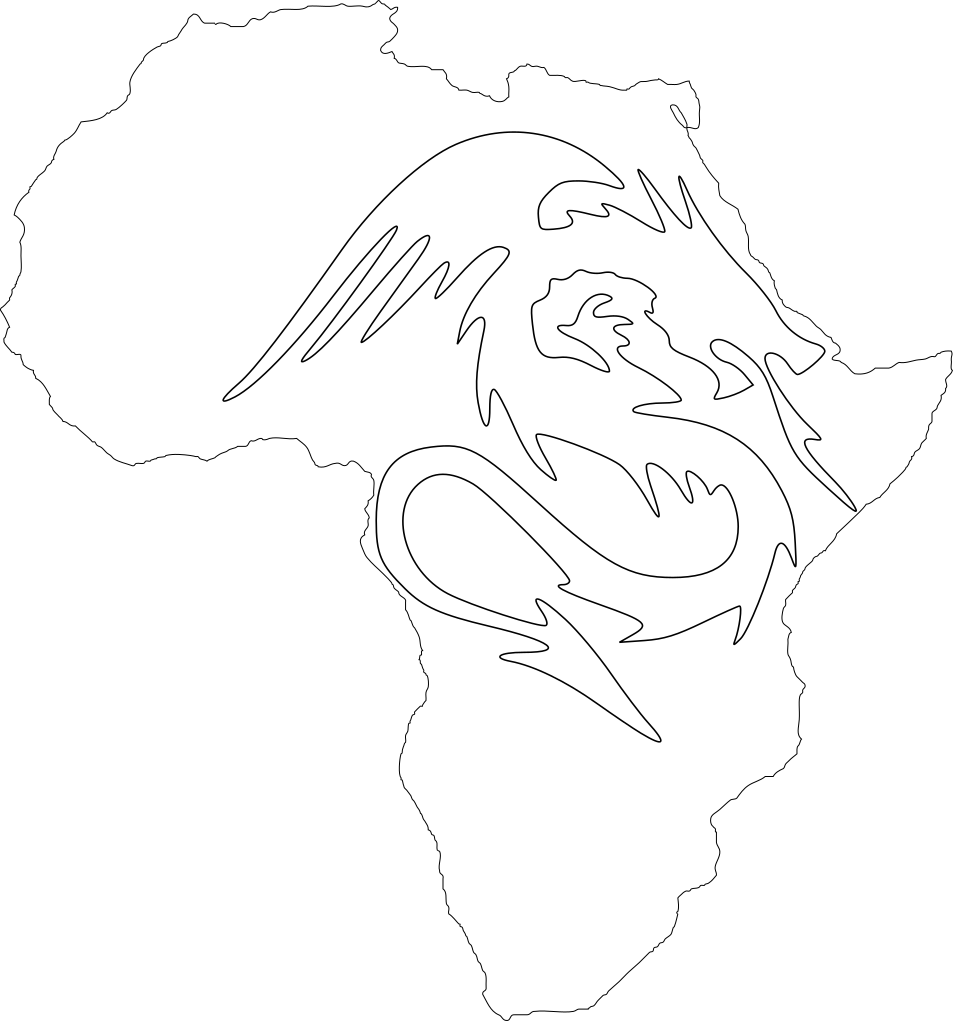
\includegraphics[width=0.5\textwidth]{images/test1_africa_dragon.png}
  \caption{На рисунки изображены 2 ломаные, состоящие из большого числа отрезков. Первая ломаная представляет собой контур Африки, вторая -- контур дракона. Видно, что эти 2 ломаные не пересекаются.}
\end{figure}

\iffalse
\section*{Вопросы:}

\begin{enumerate}

\item Назовите базовые команды командной строки linux
\item Что такое препроцессор?
\item Что делает директива \#include?
\item Что делает директива \#define?
\item Назовите все стандартные целочисленные типы C и их размер.
\item Назовите все стандартные типы с плавающей точкой в C и их размер.
\item Операторы break и continue
\item Что такое прототип функции?
\item Как функция может возвращать значения?
\item Спецификатор типа void
\item Области видимости переменных в функции
\item Передача по ссылке и по значению
\item Аргументы функции main
\item Как объявить константу в C?
\item Объявление массива
\item Как хранятся массивы в памяти
\item Строки в стиле C
\item Функции работы со строками
\item Алгоритмы сортировки вставками, выбором, пузырьком (1 из 3-х)
\item Описание структуры, typedef
\item Что такое указатель? Какой размер переменной указателя? 
\item Как получить адрес переменной? Как получить переменную по адресу?
\item Указатель на 1-й элемент массива, на 5-й.
\item Стэк и куча. Что такое, преемущества и недостатки.
\item Что делает malloc? Выделите память на массив из n элементов типа int.
\item Как освобождать память? Почему плохо не освобождать память?
\item Есть массив A состоящий из 100 элементов. Что будет, если исполнить A[110].
\item Принцип "разделяй и властвуй"
\item Сортировка слиянием или быстрая сортировка
\item Что такое связный список.
\item Сложность добавления и удаления элементов в связный список и в массив.
\item Что такое дерево?
\item Что такое двоичное дерево поиска? 
\item Сложность поиска элемента с помощью двоичного дерева поиска. Сравнение с бинарным поиском.
\end{enumerate}

\fi
\end{document}